\documentclass[a4paper,12pt,twoside]{article}

\usepackage{ucs}
\usepackage[utf8]{inputenc}
\usepackage[T1]{fontenc}
\usepackage[frenchb]{babel}
\usepackage{lmodern}
\usepackage{geometry}
\usepackage{graphicx}
\usepackage{amsmath,amssymb}
\usepackage{float} 
\usepackage{tabularx}
\usepackage{lastpage}           % numérotation
\usepackage{fancyhdr}           % en-têtes
\usepackage{verbatim}
\usepackage{mathpazo}           % police Palatino
\usepackage{xcolor}
\usepackage{listingsutf8}

% En-têtes
\pagestyle{headings}

\title{Systèmes distribués\\
  Make distribué}
\author{Bruno \textsc{Jurkovski}\and Élisabeth \textsc{Rousset}}

% \newenvironment{changemargin}[2]%
% {\begin{list}{}{%
%       \setlength{\listparindent}{\parindent}%
%       \setlength{\itemindent}{\parindent}%
%       \setlength{\leftmargin}{#1}%
%       \setlength{\rightmargin}{#2}%
%     }\item }%
%   {\end{list}}

\begin{document}

\maketitle
\newpage

\tableofcontents

\listoffigures

\newpage

\section*{Introduction}

Ce projet a pour but de programmer une version distribuée de \emph{GNU
  make}. L'exécutable créé sera désigné dans la suite de ce document
par le nom \emph{dmake}. Ce programme possède les fonctionnalités
suivantes :
\begin{itemize}
\item parsing de makefiles simples pouvant contenir des variables
\item distribution des tâches sur un ensemble de noeuds
\item transfert des fichiers nécessaires à l'exécution des tâches sur
  les noeuds concernés
\item exécution des tâches sur les noeuds
\item rapatriement des fichiers créés ou modifiés
\end{itemize}
L'archive fournie contient l'ensemble du code source compilable, les
fichiers tests ainsi que le benchmark utilisé pour l'étude de performances.

\section{Travail réalisé}

Cette section détaille les choix de conception ainsi que
l'installation et le déploiement de \emph{dmake}.

\subsection{Langage}

\emph{Dmake} est programmé en langage C++. Ce langage a été choisi
pour les raisons suivantes :
\begin{itemize}
\item Il s'agit d'un langage objet, ce qui permet d'organiser
  clairement le code et de le rendre lisible.
\item Ce langage possède de nombreuses bibliothèques optimisées qui
  facilitent la tâche du programmeur. En particulier, la gestion
  avancée des \texttt{string} est un atout pour le parsing de
  makefiles. Ce langage paraît donc plus aproprié que le C pour
  programmer \emph{dmake}.
\item Une fois compilé, un exécutable programmé en C++ est nettement
  plus rapide qu'un exécutable équivalent programmé dans un langage
  plus haut niveau comme Java. Ceci est déterminant dans la mesure où
  l'objectif de \emph{dmake} est la performance.
\end{itemize}

\subsection{Bibliothèques}

\emph{Dmake} fait appel aux bibliothèques suivantes pour la gestion
des collections :
\begin{itemize}
\item \texttt{set}
\item \texttt{map}
\item \texttt{vector}
\end{itemize}

Pour la gestion des entrées/sorties, \emph{dmake} utilise :
\begin{itemize}
\item \texttt{cstdio}
\item \texttt{iostream}
\end{itemize}

Les chaînes de caractères sont gérées à l'aide des bibliothèques
suivantes :
\begin{itemize}
\item \texttt{cstring}
\item \texttt{string}
\end{itemize}

Les flux sont gérés à l'aide de :
\begin{itemize}
\item \texttt{sstream}
\item \texttt{streambuf}
\item \texttt{fstream}
\end{itemize}

La vérification de la date de modification/création d'un fichier est
faite grâce à :
\begin{itemize}
\item \texttt{ctime}
\end{itemize}

Le déploiement et l'exécution sur les noeuds utilisent les bibliothèques :
\begin{itemize}
\item \texttt{mpi}
\item \texttt{sys/stat}
\item \texttt{cstdlib}
\item \texttt{unistd}
\item \texttt{algorithm}
\end{itemize}

\paragraph{Remarque}
Le transfert de fichiers et de tâches sur le différents noeuds est
effectué exclusivement avec les primitives de la bibliothèque MPI.

\subsection{Algorithmes}

\paragraph{Graphe de dépendances}

L'exécutable \emph{dmake} crée un graphe de dépendances orienté
acyclique pour représenter les dépendances entre les cibles du
makefile donné en entrée. Ce graphe est obtenu grâce à un tri
topologique effectué après le parsing du makefile.

\paragraph{Équilibrage de charge}

La répartion des tâches est effectuée de manière centralisée à l'aide
d'un algorithme d'ordonnancement par liste. Ce dernier s'appuie sur le
graphe de dépendances obtenu précédemment.

\subsection{Optimisations}

Deux optimisations principales ont été apportées à l'algorithme
d'ordonnancement pour améliorer les performances de \emph{dmake}.

Tout d'abord, la quantité de communications a été considérablement
réduite en forçant l'exécution de la dernière cible du makefile sur le
noeud central. En effet, il a été constaté que de manière générale, la
dernière cible (au sens du graphe de dépendances) utilise l'ensemble
des fichiers crées par les cibles précédentes.

Toujours pour réduire les communications, le choix d'un noeud pour
exécuter une nouvelle tâche prend en compte les fichiers envoyés
précédemment à ce nœud. Ainsi un nœud possédant déjà une partie des
fichier nécessaires à la nouvelle cible sera favorisé, et les fichiers
ne seront pas envoyés en double.

\subsection{Architecture}

\begin{figure}[H]
  \centering
  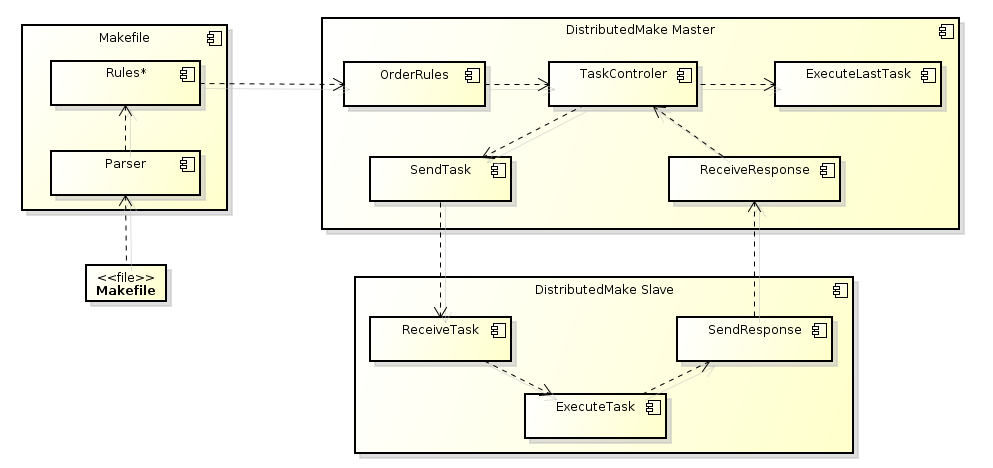
\includegraphics[scale=0.4]{schema.png}
  \caption{Architecture}
  \label{fig:architecture}
\end{figure}

\subsection{Installation}

Pour compiler \emph{dmake}, il faut se placer à la racine du
répertoire \texttt{dmake/} puis exécuter la commande :
\begin{verbatim}
> make
\end{verbatim}

\subsection{Déploiement}

Pour déployer \emph{dmake}, il faut d'abord générer la liste des
machines sur lesquelles on souhaite déployer. Pour cela on utilise le
script python \texttt{createMachines.py} en ayant préalablement indiqué
les valeurs souhaitées pour les variables \texttt{startMachine},
\texttt{NUM\_MACHINES}, et \texttt{LAST\_MACHINE} : 
\begin{verbatim}
> python createMachines.py
\end{verbatim}

Ensuite le déploiement lui-même s'effectue à l'aide de
\texttt{mpirun} (qui doit être préalablement installé sur le système). Par exemple, pour lancer \emph{dmake} sur l'un des
exemples fournis dans l'archive, il faut se placer de le dossier
contenant l'exemple puis lancer la commande :
\begin{verbatim}
> mpirun -np NB_CORES -machinefile machines.txt PATH_TO_DMAKE
\end{verbatim}


% Pour déployer \emph{dmake}, il faut tout d'abord regler les paramètre
% de déploiment dans \texttt{dmake.cfg} en indiquant le nombre de
% machines sur lesquelles on souhaite déployer \emph{dmake}, ainsi que 

\section{Tests de performances}

Les performances de \emph{dmake} ont été évaluées à l'aide d'un
benchmark programmé en C++.

\subsection{Méthodologie}

\paragraph{Configuration}
Le benchmark utilise un fichier de configuration
\texttt{benchmark.cfg} dans lequel on précise : 
\begin{itemize}
\item  le numéro de la première machine \texttt{FIRST\_MACHINE}
et de la dernière machine \texttt{LAST\_MACHINE} de l'ensemble des machines 
sur lequel on souhaite effectuer le déploiement
\item le nombre de fois
\texttt{NUM\_TIMES} qu'est répétée chaque exécution
\item Le pas \texttt{STEP} concernant le nombre de machines utilisées
  pour l'exécution
\item la localisation \texttt{PATH\_TO\_DMAKE} de \emph{dmake}
\item le répertoire d'exécution \texttt{BASE\_FOLDER}
\item le nombre de fichier tests à exécuter \texttt{NUM\_BENCHMARKS}
\item la liste des fichiers tests \texttt{BENCHMARK1}, \texttt{BENCHMARK2}\dots
\end{itemize}

\begin{verbatim}
numTimes NUM_TIMES
machines FIRST_MACHINE LAST_MACHINE
step STEP
make MAKE_TYPE
dmakeFolder PATH_TO_DMAKE
baseFolder BASE_FOLDER
numBenchmarks NUM_BENCHMARKS
BENCHMARK1
BENCHMARK2
...
\end{verbatim}

\texttt{MAKE\_TYPE} peut avoit trois valeurs :
\begin{itemize}
\item  0 : On n'exécute que le dmake.
\item  1 : On n'exécute que le make.
\item  2 : On exécute make et dmake.
\end{itemize}

\paragraph{Fonctionnement}

Le programme \emph{benchmark} fonctionne de la manière suivante : pour
chaque fichier test proposé, il exécute successivement \emph{dmake} sur un nombre de
machines allant de \texttt{FIRST\_MACHINE} à \texttt{LAST\_MACHINE}
qui est incrémenté de \texttt{STEP} machines à chaque tour. Pour un
fichier de test et un nombre de machines donnés, l'exécution est
répétée \texttt{NUM\_TIMES} fois afin d'obtenir un temps d'exécution moyen
qui soit représentatif. 
Pour chaque fichier test, le temps d'exécution moyen en fonction du
nombre de machines est écrit dans un fichier. Ce fichier est ensuite
utilisé par gnuplot pour générer la courbe correspondante. À cette
courbe est ajoutée une droite horizontale représentant le temps
d'exécution de \emph{GNU make} pour le fichier test considéré. 

\subsection{Conditions expérimentales}

Les test ont été effectués en salle D200. La salle était peu occupée
(environ 6 à 10 personnes). Cependant, les tests n'ayant pas tous été
effectués le même jour, les conditions expérimentales ont pu
varier. La charge du réseau notamment a pu être différente selon les
fichiers tests. Les makefiles utilisés pour les tests sont ceux
fournis par le professeur. Ils ont cependant subi les modifications
suivantes : 
\begin{itemize}
\item l'appel à des exécutables présents dans le répertoire courant est
  précédé d'un "./".
\item les fichiers nécessaires à l'exécution d'une cible ont été
  ajoutés dans les dépendances de celle-ci.
\end{itemize}

\subsection{Résultats et analyse}

\section*{Conclusion}
On constate que \emph{dmake} est efficace pour des makefiles dont les
tâches sont longues et relativement indépendantes
(cf. \texttt{premier}). En revanche lorsque le temps de communication
n'est plus négligeable devant le temps d'exécution des tâches, les
performances s'effondrent (cf. \texttt{matrix}). On constate le même phénomène lorsque les
tâches sont très dépendantes, car on s'approche alors d'une exécution séquentielle.






\end{document}
